% Kozierok, ch. 19
\chapter[IP subnetting: examples]{IP subnetting: practical subnet design and address determination example}
\label{chap:kozierok-ch19}

When educators ask students what they consider to be the most confusing
aspect in learning about networking, many say that it is IP address
subnetting. While subnetting isn't all that difficult in concept, it can
be a bit mind-boggling, in part due to the manipulations of binary
numbers required. Many people understand the ideas behind subnetting but
find it hard to follow the actual steps required to subnet a network.

For this reason, even though I explained the concepts behind subnetting
in detail in the previous chapter, I felt it would be valuable to have
another that provides a step-by-step look at how to perform custom
subnetting. This chapter divides subnetting into five relatively
straightforward stages that cover determining requirements; deciding how
many bits to use for the subnet ID and host ID; and then determining
important numbers such as the subnet mask, subnet addresses, and host
addresses.

My focus here is on showing the practical ``how'' of subnetting.
The topics work through two examples using a class B and a class C sample network to show you how subnetting is
done, and I am explicit in showing how everything is calculated.
This means the chapter is a bit number heavy.
Also, I try not to duplicate conceptual issues covered in the previous chapter, though a certain amount of overlap does occur.
Overall, if you are not familiar with how subnetting works at all, you will want to read the previous chapter first.
I do refer to topics in that chapter where appropriate, especially the summary tables.
Incidentally, I only cover conventional subnetting here, not variable-length subnet masking (VLSM).

This chapter may serve as a useful refresher or summary of subnetting for someone who is already familiar with the basics but just wants to review the
steps performed in subnetting.
Again, bear in mind that subnetting is based on the older, classful IP addressing scheme, and today's Internet is classless, using classless inter-domain routing (CIDR; see \vref{chap:kozierok-ch20}).

\begin{note}
If in reading this chapter, you find yourself wanting to do binary-to-decimal conversions or binary math, remember that most
versions of Windows (and many other operating systems) have a calculator program that incorporates scientific functions.
\end{note}

When you are building or upgrading a network as a whole, the first step
isn't buying hardware, or figuring out protocols, or even design. It's
{\emph{requirements analysis}}, the process of determining what it is
the network needs to do. Without this foundation, you risk implementing
a network that may perfectly match your design, but not meet the needs
of your organization. The same rule applies to subnetting as well.
Before you look at the gory details of host addresses and subnet masks,
you must decide how to subnet the network. To do that, you must
understand the requirements of the network.

Analyzing the requirements of the network for subnetting isn't
difficult, because there are only a few issues that you need to
consider. Since requirements analysis is usually done by asking
questions, here's a list of the most important questions in analyzing
subnetting requirements:

\begin{itemize}
   \item
      What class is the IP address block?
   \item
      How many physical subnets are on the network today?
      (A \emph{physical subnet} generally refers to a broadcast domain on a LAN -- a set of hosts on a physical network bounded by routers.)
   \item
      Do you anticipate adding any more physical networks in the near future, and if so, how many?
   \item
      How many hosts do you have in the largest of the subnets today?
   \item
      How many hosts do you anticipate having in the largest subnet in the near future?
\end{itemize}


\begin{keyconcept}
To successfully subnet a network, you must begin by learning what the requirements of the network will be.
The most important parameters to determine are the number of subnets required and the maximum number of hosts needed per subnet.
Numbers should not be based on just present needs, but also take into account requirements anticipated in the near future.
\end{keyconcept}

The first question is important because everything in subnetting is
based around dividing up a class A, class B, or class C network, so you
need to know which one you are dealing with. If you are in the process
of designing a network from scratch and don't have a class A, B, or C
block yet, then you will determine which one you need based on the
approximate size of the organization.

After that, you need to determine two key numbers: how many physical
subnets you have and the maximum number of hosts per subnet. You need to
know these not only for the present network, but for the {\emph{near
future}} as well. The current values for these two numbers represent how
the network needs to be designed today. However, designing only for the
present is not a good idea.

Suppose you have exactly four subnetworks in the network now. In theory,
you could use only two bits for the subnet ID, since
2\textsuperscript{2} equals 4. However, if the company were growing
rapidly, this would be a poor choice. When you needed to add a fifth
subnet, you would have a problem!

Similarly, consider the growth in the number of hosts in a subnet. If
the current largest subnet has 60 hosts, you don't want six bits for the
host ID, because that limits you to 62 hosts. You can divide large
subnets into smaller ones, but this may just mean unnecessary additional
work.

So what is the ``near future?''
The term is necessarily vague, because it depends on how far into the future the organization wants to look.
On the one hand, planning for several years' growth can make sense, if you
have enough IP addresses to do it. On the other, you don't want to plan
too far out, since changes in the short term may cause you to completely redesign your network anyway.

After you complete the brief requirements analysis, you should know the
two critical parameters that you must have in order to subnet the
network: the number of subnets required for the network and the maximum
number of hosts per subnetwork. In using these figures to design the
subnetted network, you will be faced with the key design decision in
subnetting: how to divide the 8, 16, or 24~bits in the classful host ID
into the subnet ID and host ID.

Put another way, you need to decide how many bits to steal from the host
ID to use for the subnet ID. As I explained in the section on custom
subnet masks in the previous chapter, the fundamental trade-off in
choosing this number is as follows:

\begin{itemize}
   \item
   Each bit taken from the host ID for the subnet ID doubles the number of subnets that are possible in the network.
   \item
   Each bit taken from the host ID for the subnet ID (approximately) halves the number of hosts that are possible within each subnet on the network.
\end{itemize}

There are six possible ways this decision can be made for a class C network, as illustrated in \cref{fig:subnetting-design-trade-off}.
The relationship between the bits and the number of subnets and hosts is as follows:


\begin{figure}
   \centering
   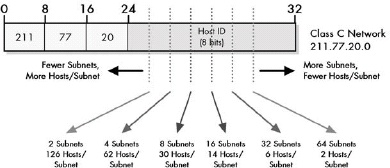
\includegraphics[width=.7\textwidth]{images/subnetting-design-trade-off.jpg}
   \caption
      [Subnetting design trade-off for class C networks]
      {Subnetting design trade-off for class C networks -- This drawing shows the options for subnetting a class C network.
      As you increase the number of bits for the host ID, you increase the number of subnets, but decrease the size of each.}
   \label{fig:subnetting-design-trade-off}
\end{figure}


\begin{itemize}
   \item
      The number of subnets allowed in the network is two to the power of the number of subnet ID bits.
   \item
      The number of hosts allowed per subnet is two to the power of the number of host ID bits, less two.
\end{itemize}

You subtract two from the number of hosts in each subnet to exclude the
special meaning cases where the host ID is all zeros (network address) or all ones (broadcast address).
As I explained in the previous chapter, this exclusion was originally also applied to the subnet ID, but is no longer in newer systems.

To choose how many bits to use for the subnet, you could use trial and error.
By this, I mean you could try to first calculate the number of subnets and hosts when you use one bit for the subnet ID and leave the rest for the host ID.
You could then try with two bits for the subnet ID, and then try with three, and so on.
This would be silly, however; it's time-consuming and makes it hard for you to choose the best option.
There's an easier method: You can use the subnetting summary tables, presented in the previous chapter.
They let you look at all the options, and you can usually see immediately the best one for you.

\section{Class C subnetting design example}

Let's take an example.
Suppose you have a class C network, with base address 211.77.20.0, and you need a total of seven subnets.
This means you need at least three bits for the subnet ID, as $2^3=8\geqslant 7$.
The maximum number of hosts per subnet is 25, which requires five bits for the host ID ($2^5 = 32 \geqslant 25$).
As $3+5=8$ this fits perfectly in a class C network.
%Looking at the subnetting summary table for class C (Table~18--5 in Chapter~18), the answer is instantly clear: You need three bits for the subnet ID.
%Why?
%This allows you eight subnets and 30 hosts per subnet.
If you try to choose two bits, you can't define enough subnets (only four).
As \cref{fig:subnetting-class-c-options} shows, if you choose four bits for the subnet ID, then you can have only 14 hosts per subnet.

 
\begin{figure}
   \centering
   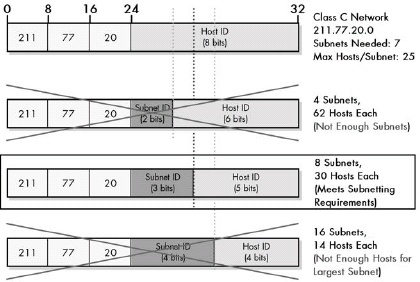
\includegraphics[width=.8\textwidth]{images/subnetting-class-c-options.jpg}
   \caption
      [Example of class C subnetting]
      {Example of class C subnetting --
      In this particular example, where seven subnets are needed and 25 hosts are needed for the largest subnet,
      there is only one choice of subnet ID size that meets the requirements. It's an easy decision!}
   \label{fig:subnetting-class-c-options}
\end{figure}

\section{Class B subnetting design example}

In some cases, especially with larger networks, you may have multiple choices.
Consider, as a more interesting example, the larger class B network 166.113.0.0, where you have a total of 15 subnets and the largest has 450 hosts.
%Examining the subnet summary table for class B (Table~18-4 in Chapter~18) suggests four acceptable options, as shown in Figure~19-3.
Using trial and error or a subnetting lookup table, one can determine four acceptable options, as shown in \cref{fig:subnetting-class-b-options}.


\begin{figure}
   \centering
   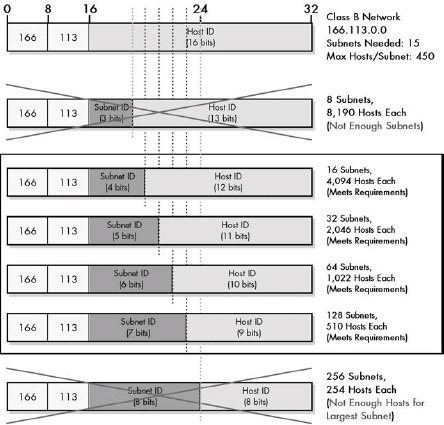
\includegraphics[width=.8\textwidth]{images/subnetting-class-b-options.jpg}
   \caption
      [Example of class B subnetting]
      {Example of class B subnetting --
      This class B network needs at least 15 subnets and must allow up to 450 hosts per subnet.
      Three subnet ID bits are too few, and eight bits means only 254 hosts per subnet, which is insufficient.
      This leaves four acceptable options, so you must choose wisely.}
   \label{fig:subnetting-class-b-options}
\end{figure}


In all four of these options, the number of subnets is equal to 15 or greater, and the number of hosts per subnet is over 450.
So which option should you choose?
Usually, you want to pick something in the middle.
If you use four bits for the subnet ID, this gives you a maximum of only 16 subnets, which limits growth in the number of subnets, since you already have 15.
The same applies to the choice of seven bits for the subnet ID, since you already have 450 hosts in one subnet now, and that limits you to 510.
Thus, you probably want either five or six bits here.
If you expect more growth in the number of hosts in the largest subnet, you
should choose five bits; if you expect more growth in the number of
subnets, you should choose six bits. If you're unsure, it's probably
best to assume more growth in the number of hosts per subnet, so here you would choose five bits.

The converse problem may also occur: You may be in a position where
there don't appear to be any options -- no rows in the summary table
match. For example, if the class C example had 35 hosts in the largest
subnet instead of 25, you would be out of luck, because there is no
combination of subnet ID and host ID size that works. The same is true
in the class B example if you had 4,500 hosts in that big subnet instead
of 450. In this situation, you would need to divide the large subnet
into a smaller one, use more than one IP address block, or upgrade to a
larger block.

 

\begin{keyconcept}
If there is more than one combination of subnet ID and host ID sizes that will meet requirements,
try to choose a middle-of-the-road option that best anticipates future growth requirements.
If no combination meets the requirements, the requirements have to change!
\end{keyconcept}
 

Once you have decided how many bits to use for the subnet ID and how
many to leave for the host ID, you can determine the custom subnet mask
for the network. Now, don't go running for cover on me. A lot of
people's eyes glaze over at mention of the subnet mask, but it's really
quite simple to figure out once you have done the homework in making the
design decision you did in step 2. In fact, there are two ways of doing
this; one is less work than the other, but they're both quite easy. I
was going to call them the hard way and the easy way, but instead, I'll
call them easy and easier.

\section{Calculating the custom subnet mask}

Let's start with the easy method, in which you calculate the subnet mask
in binary form from the information you already have about the network,
and then convert the mask to decimal. To refresh your memory and guide
the process, remember this: The subnet mask is a 32-bit binary number
where a one represents each bit that is part of the network ID or subnet
ID, and a zero represents each bit of the host ID.

\subsection{Class C custom subnet mask calculation example}

Refer back to the class C example in the previous section (\vref{fig:subnetting-class-c-options}).
Say you decided%
   \footnote{There is not much to decide if it is your only option.}
to use three bits for the subnet ID, leaving five bits for the host ID.
Here are the steps you will follow to determine the custom subnet mask for this network (illustrated in \cref{fig:determining-custom-subnet-c}):


\begin{figure}
   \centering
   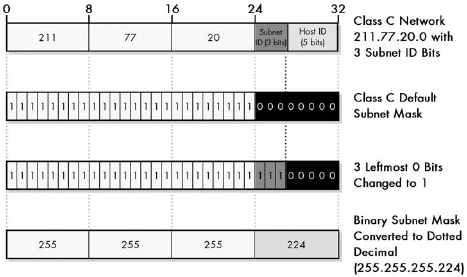
\includegraphics[width=.8\textwidth]{images/determining-custom-subnet-c.jpg}
   \caption{Determining the custom subnet mask for a class C network}
   \label{fig:determining-custom-subnet-c}
\end{figure}


\begin{enumerate}
   \item
      \textsc{Determine the default subnet mask}:
      Each of classes A, B, and C has a default subnet mask, which is the subnet mask for the network prior to subnetting.
      It has a one for each network ID bit and a zero for each host ID bit.
      For class C, the subnet mask is 255.255.255.0. In binary, this is:
      \begin{quote}
         1111 1111\quad 1111 1111\quad 1111 1111\quad 0000 0000
      \end{quote}

   \item
      \textsc{Change the leftmost zeros to ones for the subnet bits}:
      You have calculated you need three bits for the subnet ID.
      The subnet mask must have a one for each of the network ID or subnet ID bits.
      The network ID bits are already one from the default subnet mask, so,
      you change the three \emph{leftmost} zero bits in the default subnet mask from a 0 to 1, as shown in bold here.
      This results in the following custom subnet mask for the network:
      \begin{quote}
      1111 1111\quad 1111 1111\quad 1111 1111\quad \textbf{000}0 0000
      \end{quote}
      
   \item
      \textsc{Convert the subnet mask to dotted decimal notation}:
      You take each of the octets in the subnet mask and convert it to decimal.
      The result is the custom subnet mask in the form you usually see it: 255.255.255.\textbf{224}.

   \item
      \textsc{Express the subnet mask in slash notation}:
      Alternatively, you can express the subnet mask in \emph{slash notation}.
      This is just a slash followed by the number of ones in the subnet mask: 255.255.255.224 is equivalent to /27.
\end{enumerate}


\subsection{Class B custom subnet mask calculation example}

Now let's do the same example with the class B network (166.113.0.0)
with five bits for the subnet ID (with a bit less narration this time; see \cref{fig:determining-custom-subnet-b}):

\begin{enumerate}
   \item
      \textsc{Determine the default subnet mask}:
      For class B, the subnet mask is 255.255.0.0. In binary, this is:
      \begin{quote}
         1111 1111\quad 1111 1111\quad 0000 0000\quad 0000 0000
      \end{quote}

   \item
      \textsc{Change the leftmost zeros to ones for the subnet bits}:
      If you use five bits for the subnet ID, you change the five leftmost zero bits from a 0 to 1,
      as shown in bold, to give you the binary custom subnet mask, as follows:
      \begin{quote}
         1111 1111\quad 1111 1111\quad \textbf{0000 0}000\quad 0000 0000
      \end{quote}

   \item
      \textsc{Convert the subnet mask to dotted decimal notation}:
      You take each of the octets in the subnet mask and convert it to decimal to give you a custom subnet mask of 255.255.\textbf{248}.0.

   \item
      \textsc{Express the subnet mask in slash notation}:
      You can express the subnet mask 255.255.248.0 as /21, since it is 21 ones followed by 11 zeros.
      In other words, its prefix length is 21.
\end{enumerate}

 
\begin{figure}
   \centering
   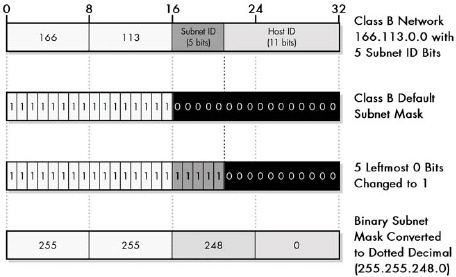
\includegraphics[width=.8\textwidth]{images/determining-custom-subnet-b.jpg}
   \caption{Determining the custom subnet mask for a class B network}
   \label{fig:determining-custom-subnet-b}
\end{figure}


\section{Determining the custom subnet mask using subnetting tables}

Now, what could be easier than that? Well, you could simply refer to the subnetting summary tables, presented in \protect\hyperlink{ch18.html}{Chapter~18}.
Find the table for the appropriate class, and then find the row that you selected in the previous step that matches the number of subnet ID bits you want to use.
You can see the matching subnet mask right there.

(Hey, it's good to know how to do it yourself! You may not always have tables to refer to!)

 

The network ID assigned to the network applies to the entire network.
This includes all subnets and all hosts in all subnets. Each subnet,
however, needs to be identified with a unique {\emph{subnet
identifier}}, or {\emph{subnet ID}}, so it can be differentiated from
the other subnets in the network. This is the purpose of the subnet ID
bits that you took from the host ID bits in subnetting. After you have
identified each subnet, you need to determine the address of each
subnet, so you can use this in assigning hosts specific IP addresses.

This is another step in subnetting that is not really hard to understand
or do. The key to understanding how to determine subnet IDs and subnet
addresses is to always work in binary form, and then convert to decimal
later. You will also look at a shortcut for determining addresses in
decimal directly, which is faster but less conceptually simple.

\begin{note}
I assume in this description that you will be using the all-zeros and all-ones subnet numbers.
In the original RFC~950 subnetting system, those two subnets are not used, which changes most of the following calculations.
See \cref{chap:kozierok-ch18} for an explanation.
\end{note}


You number the subnets starting with 0, and then 1, 2, 3, and so on, up to the highest subnet ID that you need.
You determine the subnet IDs and addresses as follows:
\begin{description}
   \item[Subnet ID]
      This is just the subnet number, and it can be expressed in either binary or decimal form.
   \item[Subnet address]
      This is the address formed by taking the address of the network as a whole and substituting the (binary) subnet ID for the subnet ID bits.
      You need to do this in binary, but only for the octets where there are subnet ID bits;
      the ones where there are only network ID bits or only host ID bits are left alone.
\end{description}
Seem complicated? Let's go back to the examples, and you'll see that it really isn't.


\section{Class C subnet ID and address determination example}

You'll recall the class C example network, 211.77.20.0.
The network address in binary is as follows:
\begin{quote}
1101 0011\quad 0100 1101\quad 0001 0100\quad 0000 0000
\end{quote}

You are subnetting using three bits for the subnet ID, leaving five bits for the host ID.
Now let's see the network address with the subnet bits in bold:

\begin{quote}
1101 0011\quad 0100 1101\quad 0001 0100\quad \textbf{000}0 0000
\end{quote}

These are the bits that you substitute with the subnet ID for each
subnet. Notice that since the first three octets contain network ID
bits, and the network ID is the same for every subnet, they never
change. You don't even really need to look at them in binary form,
though for clarity, you will do so here.

Here's how you determine the subnet IDs and addresses, again, starting with~0 (see \cref{fig:class-c-subnet-addresses}):
\begin{description}
   \item[Subnet 0]
      This has a subnet ID of 0, or 000 in binary.
      To find the address, you start with the network address in binary and substitute 000 for the subnet ID bits.
      Well gee, those bits are already all zero!
      What this means is that the address for subnet 0 is the same as the address for the network as a whole: 211.77.20.0.
      This is always the case: subnet 0 always has the same address as the network.

   \item[Subnet 1]
      This has a subnet ID of 1 in decimal or 001 in binary.
      To find the address, you substitute 001 for the subnet ID bits, which yields the following:
      \begin{quote}
         1101 0011\quad 0100 1101\quad 0001 0100\quad \textbf{001}0 0000
      \end{quote}
      Converting to decimal, you get 211.77.20.\textbf{32}.

   \item[Subnet 2]
      This has a subnet ID of 2, or 010 in binary.
      To find its address, you substitute 010 for the subnet ID bits, to give you the following:
      \begin{quote}
         1101 0011\quad 0100 1101\quad 0001 0100\quad \textbf{010}0 0000
      \end{quote}
      Converting to decimal, you get 211.77.20.\textbf{64}.

   \item[Subnet 3]
      This has a subnet ID of 011.
      As you can see, the first three octets of the address are always 211.77.20.
      The last octet here is \textbf{011}0~0000, which is 96 in decimal, so the whole address is 211.77.20.96.

      Starting to see a pattern here?
      Yes, the address of any subnet can be found by adding 32 to the last octet of the previous subnet.
      This pattern occurs for all subnetting choices; the increment depends on how many bits you are using for the subnet ID.
      Here, the increment is 32, which is $2^5$; 5 is the number of host ID bits left after you took three subnet ID bits.

   \item[Subnet 4]
      This has a subnet ID of 100.
      Its address is 211.77.20.128.

   \item[Subnet 5]
      This has a subnet ID of 101.
      Its address is 211.77.20.160.

   \item[Subnet 6]
      This has a subnet ID of 110.
      Its address is 211.77.20.192.

   \item[Subnet 7]
      This has a subnet ID of 111.
      Its address is 211.77.20.224.
\end{description}
 

\begin{figure}
   \centering
   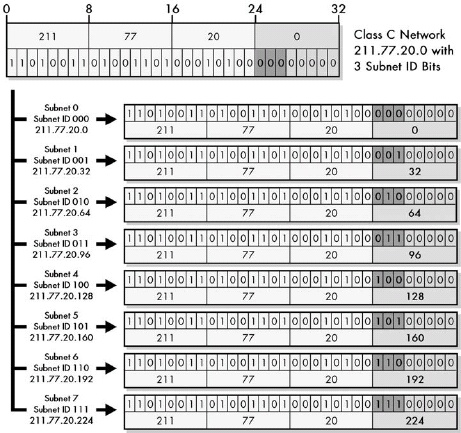
\includegraphics[width=\textwidth]{images/class-c-subnet-addresses.jpg}
   \caption
      [Determining subnet addresses for a class C network]
      {Determining subnet addresses for a class C network --
      This diagram shows each of the eight possible subnets created when you use three bits for the subnet ID in a class C network.
      The binary subnet ID is simply substituted for the subnet bits, and the resulting 32-bit number is converted to dotted decimal form.}
   \label{fig:class-c-subnet-addresses}
\end{figure}


\begin{keyconcept}
The subnet addresses in a subnetted network are always evenly spaced numerically, with the spacing depending on the number of subnet ID bits.
\end{keyconcept}

This example needed only seven subnets, 0 through 6.
Subnet 7 would be a spare.
Notice that the last subnet has the same last octet as the subnet mask for the network?
That's because I substituted 111 for the subnet ID bits, just as in the subnet mask calculation.



\section{Class B subnet ID and address determination example}

Let's look at the other example now, class B network 166.113.0.0.
In binary this is as follows:
\begin{quote}
1010 0110\quad 0111 0001\quad 0000 0000\quad 0000 0000
\end{quote}

You're using five bits for the subnet ID, leaving 11 host ID bits.
The network address with the subnet ID bits highlighted is as follows:
\begin{quote}
1010 0110\quad 0111 0001\quad \textbf{0000 0}000\quad 0000 0000
\end{quote}

Here, only the third octet will ever change for the different subnets.
The first two will always be 166.113, and the last octet will always be
0. There are 32 possible subnets; I'll list the first few so you can see
the pattern (refer to
\protect\hyperlink{ch19s04.htmlux5cux23determining_subnet_addresses_for_a-id001}{Figure~19-7}
as well):

{\textbf{Subnet 0}} This has a subnet ID of 00000. This means the
address will be 166.113.0.0, which is the network address, as you would
expect.

{\textbf{Subnet 1}} This has a subnet ID of 00001. The address becomes

\begin{longtable}[]{@{}l@{}}
\toprule
\endhead
10100110 01110001 {\textbf{00001}}000 00000000\tabularnewline
This is 116.113.8.0 in decimal.\tabularnewline
\bottomrule
\end{longtable}

{\textbf{Subnet 2}} This has a subnet ID of 00010, giving an address of
116.113.{\textbf{00010}}000.0 or 116.113.16.0.

{\textbf{Subnet 3}} This has a subnet ID of 00011 and a subnet address
of 116.113.24.0.

 

 
%\includegraphics{httpatomoreillycomsourcenostarchimages287839.png.jpg}

Figure~19-7.~Determining subnet addresses for a class B network This is
the same as
\protect\hyperlink{ch19s04.htmlux5cux23determining_subnet_addresses_for_a_class}{Figure~19-6},
but for a class B network with five subnet ID bits (I have not shown all
32 subnets, for obvious reasons).

 Again, the
pattern here is obvious: You add eight to the third octet to get
successive addresses. The last subnet here is 31, which has a subnet
address of 116.113.248.0, which has the same third and fourth octets as
the subnet mask of 255.255.248.0.




\section{Using subnet address formulas to calculate subnet addresses}

 Since the
subnet addresses form a pattern, and the pattern depends on the number
of subnet ID bits, it is possible to express the subnet addresses using
a single formula for each subnetting option. I have shown these formulas
for each of the Classes A, B, and C in the subnetting summary tables in
\protect\hyperlink{ch18.html}{Chapter~18}. The formulas can be used to
directly calculate the address of subnet {\emph{N}}, where {\emph{N}} is
numbered from 0 up to one less than the total number of subnets, as I
have done earlier.

In these formulas, the network ID bits are shown as x., x.y., or x.y.z.
for the three classes. This just means that the subnet addresses have as
those octets whatever the numbers are in those octets for the network
address. In the examples, x.y would be 166.113 for the class B network,
and x.y.z would be 211.77.20 for the class C network.

When the number of subnet bits is eight or less, the formula is
relatively simple, and a calculation is done for only one octet, as a
multiplication of {\emph{N}}, such as {\emph{N}}*4 or {\emph{N}}*32.
This is usually the case, since the number of subnets is usually less
than 256, and it's the case with both of the examples.

In the class C network with three subnet ID bits, the formula from the
table is x.y.z.{\emph{N}}*32. For this network, all subnets are of the
form 211.77.20.{\emph{N}}*32, with {\emph{N}} going from zero to seven.
So, subnet 5 is 211.77.20.(5*32), which is 211.77.20.160, as you saw
before. Similarly, in the class B network with five subnet ID bits, the
formula is x.y.{\emph{N}}*8.0. In this case, x.y is 166.113. Subnet 26
would have the address 166.113.(26*8).0, or 166.113.208.0.

This is pretty simple stuff, and it makes the formulas a good shortcut
for quickly determining subnet addresses, especially when there are many
subnets. They can also be used in a spreadsheet.

The only place where using the formulas requires a bit of care is when
the number of subnet bits is nine or more. This means that the subnet
identifier crosses an octet boundary, and this causes the formula to
become more complex.

When the number of subnet bits is greater than eight, some of the octets
are of the form {\emph{N}} divided by an integer, such as {\emph{N}}/8.
This is an integer division, which means divide {\emph{N}} by 8, keep
the integer part, and drop the fractional part or remainder. Other
octets are calculated based on the modulo of {\emph{N}}, shown as
{\emph{N}}\%8. This is the exact opposite: It means divide {\emph{N}} by
8, drop the integer, and keep the remainder. For example, 33/5 in
integer math is 6 (6 with a remainder of 3, drop the remainder, or
alternately, 6.6, drop the fraction), and 33\%5 is 3 (6 with a remainder
of 3, drop the 6, keep the remainder).

Let's take as an example the class B network and suppose that for some
strange reason you decided to use ten bits for the subnet ID instead of
five. In this case, the formula is x.y.{\emph{N}}/4.(N\%4)*64. Subnet 23
in this case would have the address 166.113.23/4.(23\%4)*64. The 23/4
becomes just 5 (the fractional .75 is dropped). 23 modulo 4 is 3, which
is multiplied by 64 to get 192. So the subnet address is 166.113.5.192.
Subnet 709 would be 116.113.709/4.(709\%4)*64, which is 116.113.177.64.

Okay, now for the real fun! If you subnet a class A address using more
than 16 bits for the subnet ID, you are crossing {\emph{two}} octet
boundaries, and the formulas become very \ldots{} interesting, involving
both integer division {\emph{and}} modulo. Suppose you were in charge of
class A address 21.0.0.0 and decide to subnet it. However, you sat down
to do this after having had a few stiff ones at the office holiday
party, so your judgment is a bit impaired. You decide that it would be a
great idea to choose 21 bits for the subnet ID, since you like the
number 21. This gives you a couple million subnets.

The formula for subnet addresses in this case is rather long and
complicated: x.{\emph{N}}/8192.({\emph{N}}/32)\%256.({\emph{N}}\%32)*8.
Yikes. Well, this is a bit involved -- so much so that it might be easier
to just take a subnet number and do it in binary, the long way. But
let's take an example and see how it works for, say, subnet 987654. The
first octet is 21. The second octet is 987654/8192, integer division.
This is 120. The third octet is (987654/32)\%256. The result of the
division is 30864 (you drop the fraction). Then you take 30864\%256,
which yields a remainder of 144. The fourth octet is (987654\%32)*8.
This is 6*8 or 48. So subnet address 987654 is 21.120.144.48.

(Don't drink and drive. Don't drink and subnet either.)

 

Once you know the addresses of each of the subnets in the network, you
use these addresses as the basis for assigning IP addresses to the
individual hosts in each subnet. You start by associating a subnet base
address with each physical network (since at least in theory, the
subnets correspond to the physical networks). You then sequentially
assign hosts particular IP addresses within the subnet (or in a
different manner, if you prefer!).

Determining host addresses is really quite simple once you know the
subnet address. All you do is substitute the numbers 1, 2, 3, and so on
for the host ID bits in the subnet address. You must do this in binary
and then convert the address to decimal form. Again, you can take some
shortcuts once the rather obvious pattern of how to assign addresses
emerges. You'll look at those near the end of the chapter.




\section{Class C host address determination example}

Let's start with the class C example again, 211.77.20.0, which you
divided into eight subnets using three subnet bits. Here's how the
address appears with the subnet bits shown in bold, and the host ID bits
shown in italics:

\begin{longtable}[]{@{}l@{}}
\toprule
\endhead
11010011 01001101 00010100 {\textbf{000}}{00000}\tabularnewline
\bottomrule
\end{longtable}

The first subnet is subnet 0, which has all zeros for those subnet bits,
and thus the same address as the network as a whole: 211.77.20.0. You
substitute the numbers 1, 2, 3, and so on for the italicized bits to get
the host IDs. (Remember that you don't start with zero here because for
the host ID, the all-zeros and all-ones binary patterns have special
meaning). So it goes like this:

The first host address has the number 1 for the host ID, or 00001 in
binary. So it is as follows:

\begin{longtable}[]{@{}l@{}}
\toprule
\endhead
11010011 01001101 00010100 {\textbf{000}}{00001}\tabularnewline
\bottomrule
\end{longtable}

In decimal, this is 211.77.20.1.

The second host address has the number 2 for the host ID, or 00010 in
binary. Its binary value is as follows:

\begin{longtable}[]{@{}l@{}}
\toprule
\endhead
11010011 01001101 00010100 {\textbf{000}}{00010}\tabularnewline
\bottomrule
\end{longtable}

In decimal, this is 211.77.20.2.

I'm sure you get the picture already; the third host will be
211.77.20.3, the fourth 211.77.20.4, and so on. There is a maximum of 30
hosts in each subnet, as you saw earlier. So the last host in this
subnet will be found by substituting 30 (11110 in binary) for the host
ID bits, resulting in a decimal address of 211.77.20.30.

You can do the same thing for each of the other subnets; the only thing
that changes is the values in the subnet ID bits. Let's take subnet 6,
for example. It has 110 for the subnet bits instead of 000. So its
subnet base address is 211.77.20.192, or

\begin{longtable}[]{@{}l@{}}
\toprule
\endhead
11010011 01001101 00010100 {\textbf{110}}{00000}\tabularnewline
\bottomrule
\end{longtable}

You assign hosts to this subnet by substituting 00001, then 00010, then
00011 for the host ID bits as shown earlier. Let's take the hosts one at
a time:

The first host address is as follows:

\begin{longtable}[]{@{}l@{}}
\toprule
\endhead
11010011 01001101 00010100 {\textbf{110}}{00001}\tabularnewline
\bottomrule
\end{longtable}

or 211.77.20.193.

The second host address is

\begin{longtable}[]{@{}l@{}}
\toprule
\endhead
11010011 01001101 00010100 {\textbf{110}}{00010}\tabularnewline
\bottomrule
\end{longtable}

or 211.77.20.194.

And so on, all the way up to the last host in the subnet, which is
211.77.20.222.
\protect\hyperlink{ch19s05.htmlux5cux23determining_host_addresses_for_a_class_c}{Figure~19-8}
shows graphically how subnet and host addresses are calculated for this
sample network.

One more address you may wish to calculate is the broadcast address for
the subnet. This is one of the special cases, as discussed in
\protect\hyperlink{ch18.html}{Chapter~18}, found by substituting all
ones for the host ID. For subnet 0, this would be 211.77.20.31. For
subnet 6, it would be 211.77.20.223. That's pretty much all there is to
it.

 

 
%\includegraphics{httpatomoreillycomsourcenostarchimages287841.png.jpg}

Figure~19-8.~Determining host addresses for a class C network This
diagram shows how both subnet addresses and host addresses are
determined in a two-step process. The subnet addresses are found by
substituting subnet ID values (shown in bold) for the subnet ID bits of
the network. Then, for any given subnet address, you can determine a
host address by substituting a host number (shown in bold and
italicized) for the host ID bits within that subnet. So, for example,
host 2 in subnet 6 has 110 for the subnet ID and 00010 for the host ID,
resulting in a final octet value of 11000010, or 194.

\section{Class B host address determination example}

 You can do
the same thing for the class B network, naturally. The address of that
network is 166.113.0.0. Now say you want to define the hosts that go in
subnet 13. You substitute 13 in binary (01101) for the subnet ID bits to
get the following subnet address, which is shown with the subnet ID bits
in bold and the host ID bits in italics:

\begin{longtable}[]{@{}l@{}}
\toprule
\endhead
10100110 01110001 {\textbf{01101}}{000 00000000}\tabularnewline
\bottomrule
\end{longtable}

This is the subnet address 166.113.104.0. Now you have 11 bits of host
ID, so you can have a maximum of 2,046 hosts. The first is found by
substituting 000 00000001 for the host ID bits, which gives an address
of 166.113.104.1. The second host is 166.113.104.2, and so on. The last
is found by substituting 111 11111110, which gives an address of
166.113.111.254. Note that since the host ID bits extend over two
octets, two octets change as you increment the host ID, unlike the Class
C example. The broadcast address is 166.113.111.255.


{\textbf{KEY CONCEPT}} In a subnetted network, the address of Host H
within subnet number {\emph{S}} is found by plugging in the binary value
of {\emph{S}} for the network's subnet ID bits, and the binary value of
{\emph{H}} for the subnet's host ID bits.

\section{Shortcuts for Computing Host Addresses}

  As
you can see, defining the host IDs is really quite straightforward. If
you can substitute bits and convert to decimal, you have all you need to
know. You can also see that, as was the case with defining the subnet
addresses, there are patterns that you can use in defining host IDs and
understanding how they work. These generally define ways for which you
can more quickly determine certain host addresses by working directly in
decimal instead of bothering with binary substitutions. This is a bit
more complex conceptually, so proceed only if you are feeling a bit
brave.

The following are some of the shortcuts you can use in determining host
IP addresses in a subnet environment:

{\textbf{First Host Address}} {\emph{The first host address is always
the subnet address with the last octet incremented by 1}}. So in the
class C example, subnet 3's base address is 211.77.20.96. The first host
address in subnet 3 is thus 211.77.20.97.

{\textbf{Subsequent Host Addresses}} After you find the first host
address, to get the next one, you just add one to the last octet of the
previous address. If this makes the last octet 256 (which can happen
only if there are more than eight host ID bits), you ``wrap around'' this
to zero and increment the third octet.

{\textbf{Directly Calculating Host Addresses}} If the number of host ID
bits is eight or less, you can find host {\emph{N}}'s address by adding
{\emph{N}} to the last octet's decimal value. For example, in the Class
C example, subnet 3's base address is 211.77.20.96. Therefore, host 23
in this subnet has an address of 211.77.20.119. If there are more than
eight bits in the host ID, this works for only the first 255 hosts,
after which you need to wrap around and increase the value of the third
octet. Consider again subnet 13 in the class B example, which has a base
address of 166.113.104.0. Host 214 on this subnet has address
166.113.104.0, but host 314 isn't 166.113.104.314. It is 166.113.105.58
(host 255 is 166.113.104.255, then host 256 is 166.113.105.0, and you
count up 58 more (314--256) to get to 314, 166.113.105.58).

{\textbf{Range of Host Addresses}} For a range of hosts for any subnet,
the first address is the base address of subnet with last octet
incremented by one. The last address is the base address of {\emph{next
subnet after this one}}, less two in the last octet (which may require
changing a 0 in the last octet to 254 and reducing the value of the
third octet by 1). For example, consider subnet 17 in the class B
example. Its subnet address is 166.113.136.0. The address of subnet 18
is 166.113.144.0. So the range of hosts for subnet 17 is 166.113.136.1
to 166.113.143.254.

{\textbf{Broadcast Address}} {\emph{The broadcast address for a subnet
is always one less than the base address of the subsequent subnet}}. Or
alternatively, one more than the last real host address of the subnet.
So for subnet 17 in the class B example, the broadcast address is
166.113.143.255.

Did I just confuse you? Well, remember that these are shortcuts, and
sometimes when you take a shortcut, you get lost. Just kidding; it's
really not that hard once you play around with it a bit.

In closing, remember the following quick summary when working with IP addresses in a subnet environment:

\begin{itemize}
   \item
      The network ID is the same for all hosts in all subnets and for all subnets in the network.
   \item
      The subnet ID is the same for all hosts in each subnet, but it's unique to each subnet in the network.
   \item
      The host ID is unique within each subnet.
      Each subnet has the same set of host IDs.
   \item
      Subnetting is fun! (Okay, okay, sorry\ldots)
\end{itemize}
